\documentclass[conference]{IEEEtran}  % Don't change

% You can add external packages
\usepackage{cite} % This is a package that modifies the way citations are handled and formatted, particularly useful for those writing academic or research papers where references are a key component.
\usepackage{amsmath,amssymb,amsfonts}  % packages provided by the American Mathematical Society (AMS), each offering various features particularly useful for typesetting mathematical content. 
\usepackage{algorithmic} % This package is used for typesetting algorithms
\usepackage{graphicx} % It adds support for including graphics in the document
\usepackage{textcomp} % Extra support for the text companion fonts
\usepackage{xcolor} % support for colored text and colored boxes in LaTeX documents.
\usepackage{subcaption}
\usepackage{graphicx}

% Add more external upackages if you need
% \usepackage{}

\def\BibTeX{{\rm B\kern-.05em{\sc i\kern-.025em b}\kern-.08em
    T\kern-.1667em\lower.7ex\hbox{E}\kern-.125emX}}   % Don't change
%\def\BibTeX defines a new command named \BibTeX

% add a new theorem if you need:
% \newtheorem{theorem}{Theorem}


\begin{document}

% Please add your subject
% e.g. ECM2427: Literature Review on Data Science for Dementia
\title{ECM2427: Literature Review on Virtual Reality Locomotion}


\author{\IEEEauthorblockN{Harry Taylor}
}

% to generate the title of the paper
\maketitle  % Don't change


\section{Introduction} % Don't change

With the continued mass market adoption of Virtual Reality (VR), the mismatch in physical space compared to virtual space remains a primary technical hurdle. While virtual worlds can be unlimited in scale, real-world room-scale constraints often lead to an immersion-breaking experience. This literature review aims to evaluate the methodologies for solving this problem, focusing on natural locomotion interfaces that align physical exertion with virtual displacement.

The scope of this review is delimited to physical motion-based techniques, excluding virtual movement through joysticks and teleportation, as well as mobility through Augmented Reality (AR) and Mixed Reality (MR) devices. This review follows a thematic structure, grouping research into three categories, focusing on a specific technology: (1) perceptual redirection (redirected walking), (2) mechanical gait simulation (omnidirectional treadmills), and (3) gesture-based proxies (walk-in-place). 

Sources were selected from IEEE Xplore and Google Scholar, prioritizing peer-reviewed studies published between 2020 and 2026. The identified solutions were critically analyzed based on several limiting factors such as biomechanical fidelity (the degree of accuracy of speed, force and feeling between a simulation and the same real task \cite{hilt2020biomechanical}) and visual-vestibular conflict, otherwise known as cybersickness, which results from sensory mismatch \cite{van2024sicknificant}.

\section{Review} % Don't change

\subsection{Perceptual Redirection - Redirected walking}
\begin{figure}[htbp]
    \centering
    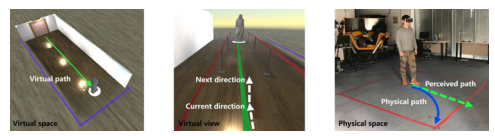
\includegraphics[width=\linewidth]{figs/path.png}
    \caption{Illustration of curvature gain used in RDW \cite{fan2022redirected}}
    \label{fig:rdw_diagram}
\end{figure}
Redirected walking (RDW) represents a software based methodology, requiring no additional hardware. In this solution, the user's perception is manipulated to steer them around physical constraints such as walls and furniture. A primary method of accomplishing this being the injection of redirection gains, introducing subtle discrepancies between the user's physical and virtual rotation, leading the user down a perceived path differing from the physical path \cite{fan2022redirected}.

A considerable factor behind the usability of this solution is the detection threshold, defining the boundaries of imperceptible manipulation of the virtual environment. An original pilot study conducted with a small 8 person group by F. Steinicke et al. \cite{steinicke2008moving} suggested that a circular path with a radius of as little as 3.3m was achievable for the majority of users in a task based environment. In contrast a more comprehensive study conducted by F. Steinicke et al. \cite{steinicke2009estimation} states a 22m radius is required before curvature is perceived in a controlled psychophysical methodology. This implies among other factors such as the rate of movement \cite{neth2012velocity}, a person's detection threshold is affected by the type of virtual environment they are exposed to. This is corroborated by a study conducted by M. Lutfallah et al. \cite{lutfallah2024revisited} on naive subjects, stating that in a VR shooting game, applying "distractors" allowed for a generally higher threshold, as the user's cognitive focus is diverted away from the redirected motion. 

A key limitation of these studies is the use of a much larger and open laboratory space. The compilation of results indicate that even with aggressive misdirection, a minimum space of $34\,\mathrm{m}^2$ is required for the system to be imperceptible. This implies for a complete non-immersion breaking experience and limited cybersickness, a space larger than the typical home room-scale space is required, leaving this solution to be only viable for large venues.

\subsection{Mechanical Gait Simulation - Omnidirectional Treadmills}
\begin{figure}[htbp]
     \centering
     \begin{subfigure}[b]{0.15\textwidth}
         \centering
         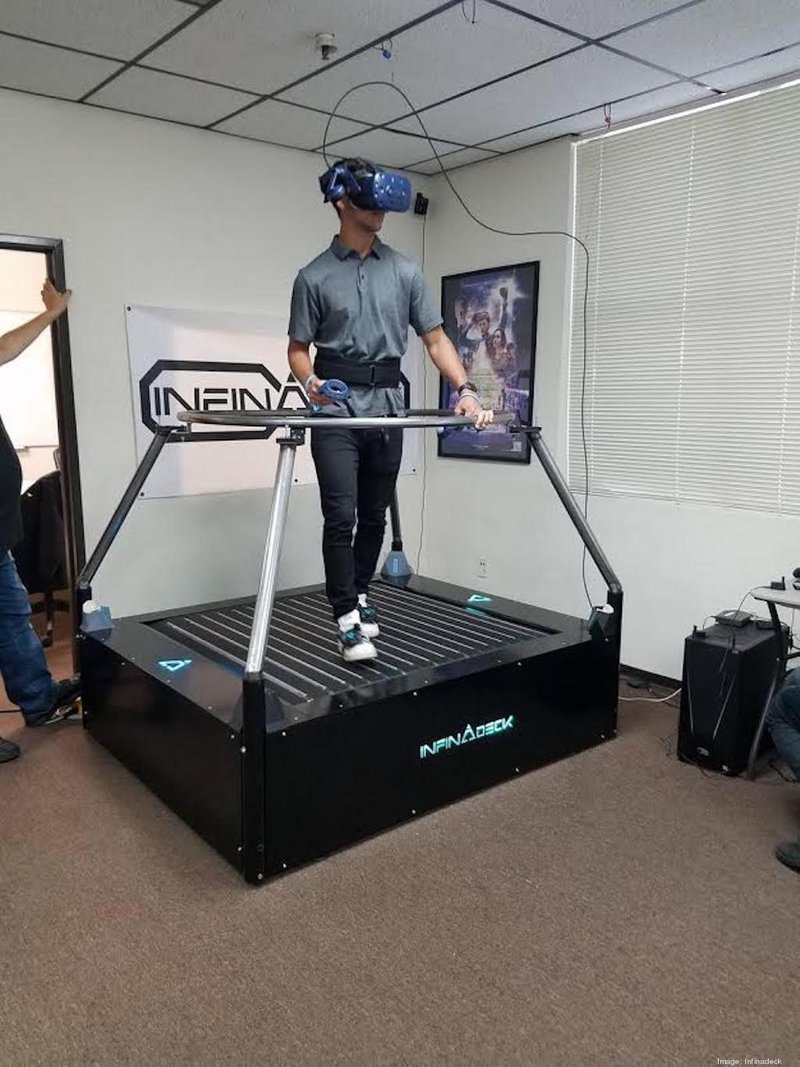
\includegraphics[width=\textwidth]{figs/active.jpg}
         \caption{Active ODT "InfinaDeck"}
         \label{fig:active}
     \end{subfigure}
     \hspace{0.5cm}
     \begin{subfigure}[b]{0.134\textwidth}
         \centering
         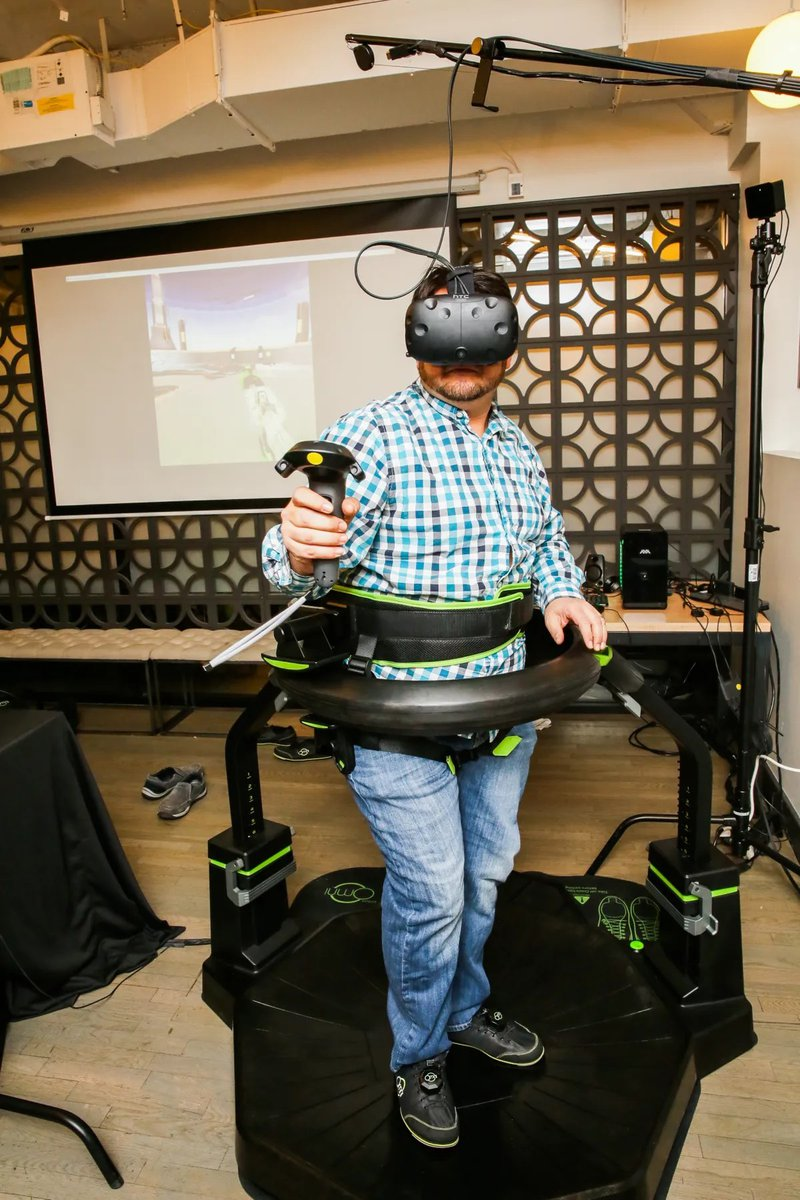
\includegraphics[width=\textwidth]{figs/passive.jpg}
         \caption{Passive ODT "Omni One"}
         \label{fig:passive}
     \end{subfigure}
     \caption{Comparison of Omnidirectional Treadmill (ODT) architectures. \cite{viveblog2024treadmills}}
     \label{fig:comparison}
\end{figure}
An alternative solution researched is omnidirectional treadmills (ODTs). These systems utilise a kinetic surface to counteract the user's velocity in real time, thereby enabling unconstrained locomotion within a stationary physical footprint \cite{wehden2021slippery}. These systems can be catagorised as active, where motorised belts or rollers dynamically respond to the users step, or passive, which employs a low friction surface to keep the user positioned at the centre of the device \cite{wang2023redirected}. Both approaches theoretically allow for 1 to 1 mapping between virtual and physical displacement, allowing for infinite navigation in a localised area.

The usability of ODTs is driven by their level of proprioceptive feedback, an internal sense of self-movement. This feedback significantly improves user presence compared to conventional joystick controls \cite{wehden2021slippery}. By engaging the user's legs, the necessary sensory cues are met between the vestibular and visual systems, theoretically mitigating cybersickness \cite{lohman2022evaluating}. Despite this benefit, biomechanical fidelity can be affected by the type of solution used. In a study conducted by A. Bashir et al. \cite{bashir2023comparing} utilising a passive ODT, users typically found it more difficult to complete the task at hand, walking with an unnatural gait and at slower speeds. However, this was only compared to a conventional unidirectional treadmill.

When considering active solutions, mechanical latency and deceleration of the surface can damage the user experience, leading to sensory mismatch and cybersickness according to Z. Wang et al. \cite{wang2022strolling}. However this study was largely based on continuous predictable walking, without considering more erratic movements, such as quick directional changes, and strafing that may be needed for high intensity VR tasks. This is alongside the technical limitations of active systems, with fully omnidirectional systems only being viable recently via multi-axis belt arrays such as the Infinadeck \cite{viveblog2024treadmills}. Previously, active systems would typically rely on two axes, with redirected walking used to emulate omnidirectional nature \cite{wang2023redirected}.

Ultimately, Mechanical gait simulation offers a direct theoretical solution to the space mismatch and cybersickness problems associated with locomotion, within a reasonable room-scale footprint of as little as $1.76m^2$ \cite{wang2022strolling}. However, the practical viability of these systems remains compromised by the biomechanical and systematic solutions previously discussed. Furthermore, a key factor frequently marginalised in current literature is the prohibitive cost and physical accessibility of this hardware, preventing widespread adoption. Even passive consumer oriented ODTs such as the Omni One Core cost from \$2,595 \cite{virtuix2026omni}.

\subsection{Gesture Based Proxies - Walking in Place}
\begin{figure}[htbp]
    \centering
    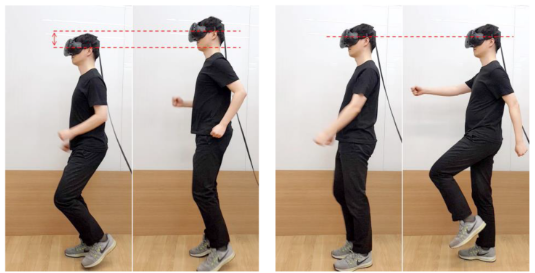
\includegraphics[width=0.9\linewidth]{figs/walking.png}
    \caption{"March in place" motion used in WIP \cite{lee2018walking}}
    \label{fig:rdw_diagram}
\end{figure}
Walking in place (WIP) has emerged as a prominent alternative for continuous virtual locomotion. WIP systems operate by tracking the user's stationary physical stepping motions. This is typically accomplished through tracking head oscillations captured by the Head-Mounted-Display (HMD), with additional optional inertial measurement units (IMUs) attached to the legs or arms for increased accuracy \cite{tregillus2016vr}.

While WIP can solve the hardware accessibility problem often associated with VR locomotion, it can introduce its own discrepancies, most notably the lack of physical forward momentum. When evaluating the efficacy of these systems, a trade-off is revealed between input accessibility and biomechanical fidelity. As demonstrated by P Hořejší et al. \cite{hovrejvsi2025virtual}, who stated while "Cybershoes" introduced lower-limb proprioception, subjects were often left with residual cybersickness, although this study limited use of Cybershoes to a seated position, partly contributing to this feeling.

However, even when systems allow for standing movement, a tradeoff arises through tracking limitations. For instance, S Tregillus et al. \cite{tregillus2016vr} introduced VR-step, a WIP method relying on smartphone IMUs for detecting step motions. While this approach demonstrated high accuracy in basic step recognition using universally available hardware, a critical weakness of this solution is its failure to account for the continuous kinematic variations of natural walking. This reliance on basic step recognition consequently contributes to noticeable start-stop latency, with many users reporting overshooting the locations they were meant to stop at. Furthermore, as the system was evaluated by its own developers, these findings are inherently susceptible to selection bias. 

To combat latency based problems, L Zhao et al. \cite{zhao2021classifying} proposed an end-to-end machine learning approach, analysing consecutive frames of user movement. This solution achieved a high 95\% classification rating, with a reduced            latency of 192ms compared to the common ~400ms half step latency of WIP systems \cite{tregillus2016vr}.

Logistically, similarly to mechanical gait simulation, theoretically the solution extends to full 1 to 1 traversal between the virtual and physical world. However, human biomechanics make stationary marching without sight or a restraint difficult. As a result, WIP solutions can cause users to unintentionally drift from their starting position \cite{nilsson2014comparison}, potentially risking collision with objects in the physical world.

\section{Conclusion} % Don't change
Bridging the gap between virtual and physical environments remains a fundamental challenge in VR locomotion. This review evaluated three prominent methodologies and the literature surrounding each. This review has revealed that the current landscape of VR locomotion is defined by a persistent compromise between spatial requirements, hardware accessibility, biomechanical fidelity and cybersickness. 

While perceptual redirection techniques offer high immersion, their reliance on massive physical footprints renders them largely unusable for the standard room scale consumer. Conversely ODTs successfully confine unencumbered movement to a footprint small enough for room-scale use, and deliver proper proprioceptive feedback. However, these systems remain critically bottlenecked by prohibitive consumer costs and mechanical latency. Finally WIP systems provide a highly accessible, highly compatible solution which can work in room scale, but fundamentally fail to replicate true acceleration, leaving users with a lack of immersion and potentially cybersickness.

Furthermore, the current adoption of consumer VR locomotion systems limits variety in research testing. Locomotion systems reviewed by sources in this report have been conducted under sterile lab conditions, leading to a lack of variety and forced limitation in use of the solutions. As a result the often brief user experience of these solution could be improved upon in further research, focusing on deploying these systems in users' homes for longer term, unrestricted use. 

Ultimately, no single methodology provides a flawless and universal solution to the VR locomotion problem, as solutions each hold their own mechanical and biological ceilings. As some papers have already tried implementing, VR locomotion may depend in future on hybrid implementations, involving mixed qualities of multiple of the solutions discussed. By synthesising these alternative solutions, the VR industry can continue to close the sensory gap between the physical and virtual worlds, moving to an unencumbered solution.

% This command sets the style in which the bibliography is formatted. You must use IEEE reference style
\bibliographystyle{ieeetr} % Do not change, it gives you the IEEE bibliography styles.

% You should add your references in the file "reference.bib"
\bibliography{reference.bib} % Do not change

\end{document}